
%(BEGIN_QUESTION)
% Copyright 2011, Tony R. Kuphaldt, released under the Creative Commons Attribution License (v 1.0)
% This means you may do almost anything with this work of mine, so long as you give me proper credit

The {\it Nernst equation} finds application in many different chemical analyzer technologies.  One of these analytical technologies is {\it oxygen concentration} in mixed gas streams, such as the exhaust from a combustion process where oxygen content is usually maintained at about 2\% (instead of the normal 20.9\% oxygen concentration of Earth's atmosphere).  A common oxygen sensor is made of a ``sandwich'' of platinum electrodes on either side of a solid zirconium oxide membrane.  One side of this electrochemical cell is exposed to the exhaust gas (process), while the other side is exposed to heated air which serves as a reference:

$$\includegraphics[width=15.5cm]{i00929x01.eps}$$

Voltage output by the cell is predicted by the Nernst equation:

$$V = {{R T} \over {nF}} \ln \left({C_1 \over C_2}\right)$$

\noindent
Where,

$V$ = Voltage produced across membrane due to ion exchange, in volts (V)

$R$ = Universal gas constant (8.315 J/mol$\cdot$K)

$T$ = Absolute temperature, in Kelvin (K)

$n$ = Number of electrons transferred per ion exchanged (2, for oxygen atoms)

$F$ = Faraday constant, in coulombs per mole (96,485 C/mol e$^{-}$)

$C_1$ = Concentration of oxygen in ambient air (20.9\%)

$C_2$ = Concentration of oxygen in exhaust gas

\vskip 10pt

Suppose a DAQ module were connected to one of these oxygen-sensing cells, and you needed to enter a formula into the DAQ software to translate voltage into oxygen concentration.  Manipulate the Nernst equation to solve for the concentration of oxygen in the exhaust gas from the measured voltage:

\vskip 30pt

$C_2$ = 

\vfil 

\underbar{file i00929}
\eject
%(END_QUESTION)





%(BEGIN_ANSWER)

This is a graded question -- no answers or hints given!

%(END_ANSWER)





%(BEGIN_NOTES)

The key to manipulating this equation to solve for $C_2$ is ``un-doing'' the natural logarithm function.  Recall that every arithmetical function has its inverse.  For addition, the inverse function is subtraction.  For multiplication, the inverse function is division.  For logarithms, the inverse function is an exponential: in this case, un-doing a natural logarithm requires we apply a power of $e$.  We see how this works in the third line:

$$V = {{R T} \over {nF}} \ln \left({C_1 \over C_2}\right)$$

$${VnF \over RT} =  \ln \left({C_1 \over C_2}\right)$$

$$e^{VnF \over RT} =  e^{\ln \left({C_1 \over C_2}\right)}$$

$$e^{VnF \over RT} =  {C_1 \over C_2}$$

$$C_2 = {C_1 \over e^{VnF \over RT}}$$

If we happen to know that each oxygen ion has a double-negative charge on it, we may replace $n$ in the equation with the number 2 for this specific application:

$$C_2 = {C_1 \over e^{2VF \over RT}}$$

%INDEX% Mathematics review: manipulating literal equations

%(END_NOTES)

